% !TeX spellcheck = en_US
\chapter{Introduction}
\section{Motivations}
In the past few decades, the digitalization of multimedia content and the diffusion of network connectivity brought an exponential growth of accessibility to such content. The wide spreading of smartphones and low-cost devices, as well as the diffusion of social networks, also led to a surprising democratization of content fruition and production. 
As things stand today, millions of webpages, images, songs and videos are just \textit{one click away} from users \cite{Buccoli2013}, which easily causes \textit{information overload}. 

The existing libraries of content have reached dimensions that require indexing through effective organization strategies, otherwise users will not be able to access them. Before the digital era and before the Internet, traditional approaches for organizing content relied on hierarchical taxonomies and manual scanning. The taxonomies included categories and subcategories, and the users needed to browse through all the content within selected subcategories. This approach was used for a number of scenarios, from the organization of books in libraries, to the indexing of websites such as the Yahoo search engine \cite{taubes1995rohtua}. This strategy, however, is no longer sufficient for the current multimedia libraries because of two main limitations: the need of manual effort to build the taxonomy, keep the content organized, and scan through the content; and the rigidity of the organization with respect to other types of taxonomy, e.g., sorting the books by year, topic or cultural movement. 

Current approaches for handling huge multimedia libraries are based on automatic systems to organize the content, and on the use of high-level descriptors to access it. These approaches overcome the limitations of the manual effort and rigidity of the taxonomies by allowing the users to \textit{scrape} the information in a more familiar and effective way. Going back to the previous examples, modern search engines allow the users to browse through the websites by looking for information (e.g., \textit{a black cat}, the animal with black fur) and its related concepts (e.g., superstition associated to a black cat, the related short story by Edgar Allan Poe). The design and development of such novel approaches, based on the high-level meaning of the content, i.e., on its semantics,  must be tailored on the type of content that is being addressed. The semantics and users' needs concerning text document are in fact different from those regarding images, or videos. In this thesis, we focus on semantics of and users' needs on musical content.

A traditional approach to organizing music was mainly based on genres and subgenres. Within the chosen subgenre, the users had to scan through the albums in order to retrieve the one that they were interested in. Some degree of "mediation" was done by the music dealer, who advised the customers on which album to choose and had the important role of narrowing down the choice of music for the customer \cite{Zanoni2013Thesis}. In the current scenarios, with million of songs to choose among, the categorization based on genres is still in use, but it is no longer sufficient and a manual scanning is no longer feasible for subcategories counting thousands of music pieces. The categorization based on genres has been assisted and being replaced by novel approaches, which include ready-to-use playlists based on some high-level descriptors of the songs \cite{maillet2009steerable}, and the automatic recommendation of new songs based on users' listening history \cite{FtHandbook}.

%The semantic domain of music is complex and concerns several aspects (mood, timbre, dynamics, etc).
The aim of this thesis is to investigate the novel semantic-based approaches for scraping the musical content, by following a \textit{schema} that generalizes such approaches. In order to do so, we need to understand the possible high-level meaning and interpretation of the musical content, i.e., its \textit{semantic domain}. The semantic domain of music concerns several aspects, including those related to the quality of the sound (e.g., the \textit{timbre}), of the performance (e.g., the \textit{dynamics}) or the elements that are rather related to the subjective response of the listeners (e.g., the \textit{mood}). Due to the high number of semantic aspects, and to the possible ambiguities of their description, the definition of the semantic domain of music is a hard task.

%However, we must retrieve musical content, by applying signal processing techniques, so we need to formalize the signal domain. 
In order to develop applications that are able to automatically organize the semantics of musical content, we must also learn to handle and manipulate the content itself, which is represented by an audio signal. We use signal processing techniques to formalize the domain of the musical content, i.e., the \textit{signal domain}, by investigating which characteristics are more effective to describe it and which techniques can be used to automatically extract such features. 

%Finally, we need to find solution to link the signal domain and the semantic domain. 

The signal domain concerns the musical content and the aspects that can be automatically extracted or inferred from it, while the semantic domain concerns the way people describe and think of music from a higher-level perspective. There is however a significant gap between the two domains, which needs to be bridged by means of a \textit{linking function} that assigns elements from the domain of a problem to the corresponding elements in the codomain. The linking function is two-directional, and its direction depends on the scenario that we aim at addressing. When used to automatically infer the high-level meaning of the musical content, the link goes from the signal to the semantic domain. When, instead, we want to enrich the musical content with high-level information, the direction of the link goes from the semantic to the signal domain.


The schema we use throughout this thesis is based on the \textit{formalization} of the signal and semantic domain and on the definition of the linking function between the two domains. We need to represent the nature of the musical content as objects that are feasible to be analyzed, and therefore formalize such representation of the signal domain. Analogously, we need to provide a formalization of the semantic domain as a representation of the users' needs. The musical properties and the users' needs are abstract entities that must be represented as analyzable concrete objects. The choice of such representation and the procedure of transformation from abstract entities to concrete objects is the actual formalization. This can be achieved through an in-depth knowledge of the nature of the music, of the user's needs, as well as the techniques that are able to bridge the gap between them. 

The formalization of the domains and the definition of the linking function for the problems related to the musical content involve several research fields, such as signal processing, psychoacoustics, musicology, psychology, computer science and machine learning. \textit{Music Information Retrieval} (MIR) \cite{muller2007information} is a multi-disciplinary research field that includes the aforementioned research fields to address the problems related to the extraction and processing of information from the musical content and the retrieval of musical items. 

Our work concerns two main steps: the definition of the components to generalize the novel scraping approaches, by exploiting and expanding the state of the art of MIR; and the application of the components within selected MIR application scenarios. For this reason, we divide our thesis in two parts that cover the two aforementioned steps. 


In the following we define the outline of the thesis and we introduce the main contributions of this work.


\section{Definition and formalization of the components of the schema}
The first part of this work is devoted to the formalization and definition of three main components, as represented in Figure \ref{fig:intro:scheme}. We explore the state of the art for the formalization of the signal and semantic domain, and we conduct two research activities to overcome possible limitations for the two tasks. We also provide an overview of the techniques proposed to define the linking function.

\begin{figure}[tbp] 
	\begin{center}
		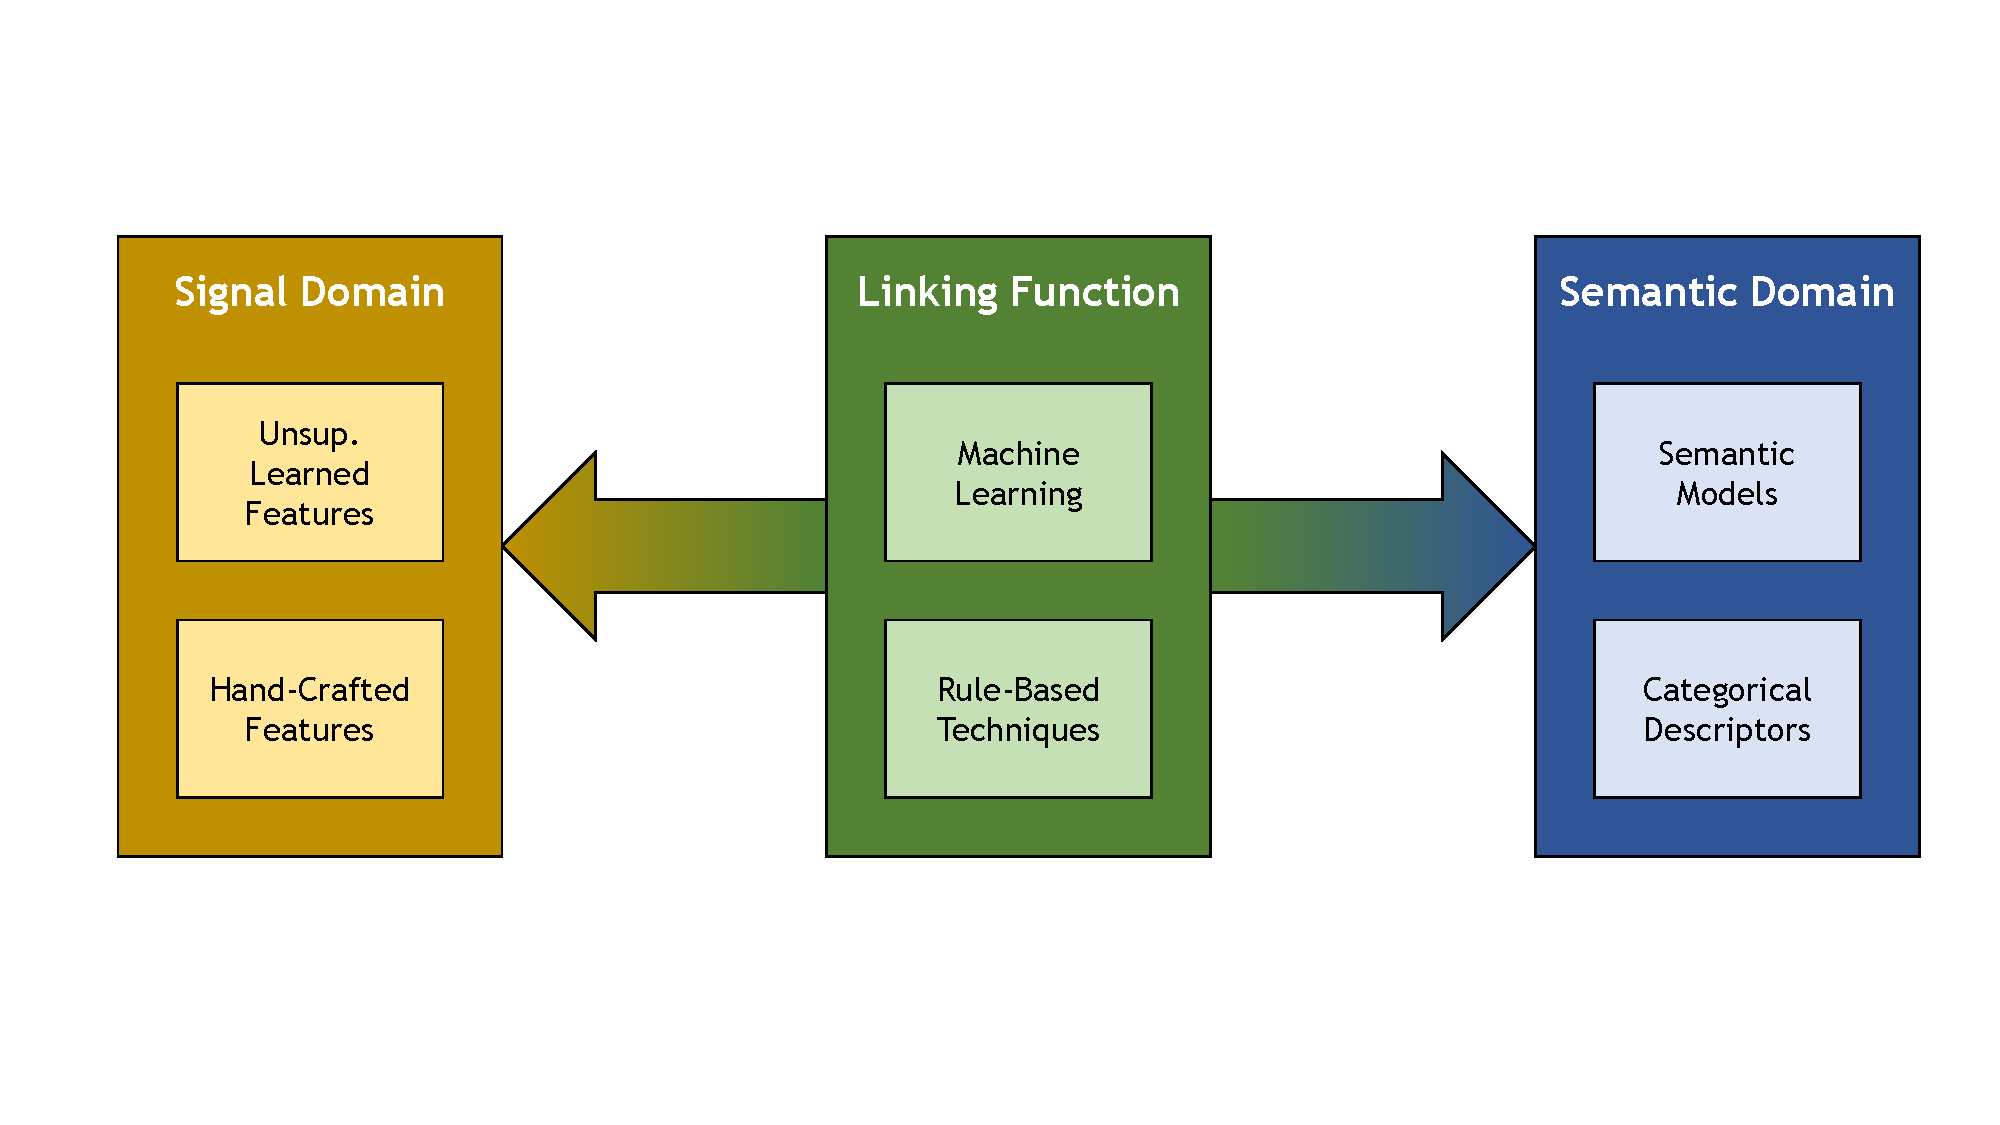
\includegraphics[trim=1.9cm 4.5cm 1.3cm 3.7cm,clip=true,width=\textwidth]{img/intro/schema_new_colorz}
		%\psfig{file=im/ML/logopm.jpg,width=3.5cm}
	\end{center}
	\caption{A visualization of the schema used throughout the thesis}
	\label{fig:intro:scheme}
\end{figure}

\subsection{Feature representation of the signal domain}
%As far as the signal domain is concerned, MIR community has proposed LLFs, MLFs and, most recently, approach based on deep learning.
The MIR literature has developed several techniques to represent the characteristics of the musical content by means of the automatic extraction of related \textit{features}. Such features are traditionally categorized by their level of abstraction from the underlying signal \cite{Celma2008}. In Chapter \ref{Chap:LLFs} we discuss the formalization of the features for the different levels of abstraction.

The lower level of abstraction is captured by the \textit{Low-Level Features} (LLFs ) \cite{Kim2004}, which extract the characteristics related to the physical nature of the audio signal. Such characteristics include the energy or the noisiness of the sound. The LLFs are extracted using clear mathematical formulations, which makes them easy to compute, highly objective, and therefore a reliable formalization for the signal domain. 

On a higher level of abstraction, there are the \textit{Mid-Level Features} (MLFs) \cite{Fu2011}, which concern the aspects of music composition and execution \cite{Muller2011}. While several models have been proposed by the MIR community, there is not a clear formulation to extract MLFs, and they are, in fact, less objective than the LLFs. 

LLFs and MLFs have been manually designed, based on signal processing techniques and studies on human perception and psychology of music. Therefore, they are named \textit{hand-crafted} or \textit{model-based} features and their interpretation is a valuable resource to infer some insight on the signal domain. In order to do so, it is important to deeply understand which aspect is captured by each feature. 

In order to develop such understanding, in Section \ref{sec:NMP} we conduct a feature-based analysis of the Networked Music Performance (NMP) task, where two or more musicians are willing to interact from different locations, by means of an Internet connection \cite{barbosa2003displaced}. Traditional literature on NMP focus on which network architecture can be used to minimize the network delay \cite{saputra2012design,gu2005network,renwick2012sourcenode}. Instead, we investigate which properties of the musical performance, and therefore which features extracted from the signal domain, affect the overall quality performance.  

In some situations, however, the definition of the signal domain is fuzzy and it is not clear which properties are more effective to characterize the domain or which feature can actually capture them. It is not possible, therefore, to address the problems related to such situations using feature-based analysis techniques. In the latest years, a novel and powerful method for feature extraction has emerged, named \textit{deep learning}, that mimic the behavior of the human brain by organizing the information in multiple hierarchical layers \cite{Haykin1998,Goodfellow2016}. Each layer provides a description of the content with different levels of abstraction.% and therefore the deep learning techniques can be used to automatically learn a feature representation of the signal domain.

One of the most interesting properties of deep learning techniques is their ability to learn the feature representation with no specific information on the aspects that need to be extracted, i.e., in an unsupervised manner. While such \textit{unsupervised learned features} have no direct interpretation, they have been proven to be more effective than the traditional hand-crafted and model-based features in several MIR tasks \cite{Hamel2010, Schmidt2011, Humphrey2013}. In Section \ref{sec:LLFs:learned} we offer an overview of the state of the art of deep learning techniques in MIR.

\subsection{Techniques to design the linking function}
%As far as the linking function is concerned, MIR community has proposed to rule-based and machine-learning techniques.

With respect to the linking function, we can use different techniques from the MIR literature, depending on the complexity of the formalization and on how wide the gap between the signal and the semantic domain is. In Chapter \ref{Chap:ML} we discuss the two main approaches for the design of the linking function: rule-based and machine learning techniques. The former strategies are manually designed and developed by researchers and therefore can be used in a limited number of cases. Rule-based techniques are commonly used when the domains are formalized well enough and there is a proper knowledge on the nature of the linking function. 

In most cases, however, the formalization of the domains is not so precise, and the semantic gap is wide, in particular when bridging the gap involves the modeling of the human perception, which is two-fold. On one side, the modeling, concerns the low-level processing of the sensory input, which is affected by the physical sound, and on the other side it involves the processing and high-level interpretation of such input \cite{Bernstein2010}. For this reason, modeling the human perception affects both the signal and the semantic domains, as well as the linking between the two. In such cases, we can use machine learning techniques, which are able to automatically learn a predictive model that links input and output domains. Machine learning techniques have been widely used in MIR tasks \cite{coviello2011,sturm2014}. In Section \ref{sec:ML:models} we provide an overview of some machine learning techniques from two traditional categories: classifiers and regressors \cite{friedman2001}. The former predict an outcome from a set of discrete values, while the latter predict an outcome within a continuous range of values. 


\subsection{Formalization of the semantic domain}
%As far as the semantic domain is concerned, MIR community has proposed classification approaches, categorical approaches, dimensional models and even ontologies.

With respect to the semantic domain, in Chapter \ref{Chap:HLFs} we discuss the so-called \textit{High-Level Features} (HLFs) \cite{Le2013} used for music description. The HLFs provide a formalization of the semantic aspects of music, such as the mood perceived in a song or its genre. However, due to their abstract nature, there is no objective mathematical formulation that we can use for extracting them.
For this reason, it is common to first formalize the semantic domain, and then to design the linking function to extract the semantic description from the musical content or retrieve the musical content from the semantic description.

There are two main approaches to the formalization of the semantic domain: the \textit{categorical} and the \textit{dimensional} \cite{Sordo2012}. The \textit{categorical} approach provides a qualitative description of music, i.e., specifies whether or not a certain feature can be used to describe a song (e.g., \textit{this song is groovy} or \textit{not groovy}). Following the categorical approach, we discuss two different types of formalizations. The former involves the definition of a set of disjoint categories for the description of the songs, while the latter allows the semantics of the descriptors to overlap, i.e., to represent a song with numerous descriptors.

The \textit{dimensional} approach provides a quantitative description, i.e., specifies the degree of descriptiveness of a feature for a song (e.g., \textit{this song is rather groovy}, which might be represented as a value of 0.7 of grooviness). While the categorical approach is easier to use, the dimensional approach supports the possibility to use a nuanced description that is more accurate and closer to the natural language. Because of this more accurate description, the dimensional approach can be used to provide a better formalization of the semantic domain and to define a \textit{semantic model}. 

In Section \ref{sec:HLFs:VA} we review a psychological model for the emotional-related descriptors, the Valence-Arosaul (VA) model \cite{Russell1980}, which involves two dimensional descriptors: \textit{Valence} describes the degree of positiveness (or negativeness) of the mood; and \textit{Arousal} is related to its degree of activation. The Valence and Arousal are in fact two high-level dimensional descriptors, which have been widely used to build a semantic model for the semantic description of the mood conveyed by music \cite{Kim2010,Weninger2014, aljanaki2015emotion}. Since such semantic model closely follows the principles of the psychological VA model, it is commonly named VA model itself. In the VA model, the emotional-related HLFs and the mood conveyed by the music pieces are represented as points in the VA space, where a metric of distance between the points can be defined to model the semantic relation between the objects. 

Given the importance of the VA model, \cite{Bradley1999} presents the ANEW dataset, which is composed of more than 2000 descriptors mapped in the VA space. While the ANEW dataset has been a valuable resource for the MIR community \cite{Kim2010,Weninger2014, aljanaki2015emotion,Yang2012, Cowie2012, Scherer2004} the dataset presents some issues, due to the fact that it is a generic dataset, and it is not tailored for music description. As an example, the distance between two descriptors in the VA space might not be effective to capture their semantic relation for music description. In order to overcome such issues, in Section \ref{sec:HLFs:ANEW} we conduct a research activity aiming at designing a novel space, drawn from the ANEW dataset, where the terms are better conceptually organized for music description. We conduct our research by shaping the novel space according to prior information on how users think of emotional-related descriptors.



% in the music context, and shaping a high-dimensional space built from the ANEW dataset accordingly to the collected information. %This processing helps us to de-clutter the dataset and to find a space where terms follows a better conceptual organization with regard to the music description.


%Second part: overview of the application scenarios
\section{Overview of the application scenarios}
The second part of this work is devoted to apply the aforementioned techniques in a number of real-world scenarios for different MIR tasks.
We gradually increase the complexity of the scenarios, i.e., the complexity of the formalization of signal and semantic domains, and of the definition of the linking function.
In Table \ref{tab:intro:chapters} we list the various application scenarios with the issues to be addressed for each of them. 

\begin{table}[tbp]
\centering
\caption{Structure of the thesis}
\label{tab:intro:chapters}
  \bgroup
  \def\arraystretch{1.5}
\begin{tabular}{||l|>{\RaggedRight}p{2.2cm} |>{\RaggedRight}p{3cm} >{\RaggedRight}p{3cm} >{\RaggedRight}p{2.8cm}||}
\hline
\hline
\textbf{Chapter}  &\textbf{Application}& \textbf{Signal domain} & \textbf{Linking Function} & \textbf{Semantic Domain} \\
\hline
\hline
Chap. \ref{Chap:MSA} & Music \newline Structure Analysis & Poorly known: learned features & Rule-based \newline techniques &  Well known \\
\hline
Chap. \ref{Chap:Bootleg} & Bootleg \newline Detection &  Poorly known: learned features    &  Machine Learning techniques  & Defined but \newline unkown \\
\hline
Chap. \ref{Chap:Violin} & Timbral \newline description of violins & Unknown: learned features    & Machine Learning techniques  & Fuzzy: \newline semantic model \\
\hline
Chap. \ref{Chap:DCSM} & Semantic model for description and retrieval & Musical content  & Information \newline Retrieval system  &  Ambiguous: \newline semantic model\\
%\hline
%Chapter 11 & Multimodal & Unkown & Highly vast \\
\hline
\hline
\end{tabular}
\egroup
\end{table}

%Our work involves the development of music virtual mediators as a linking function between the music physical domain and the user semantic codomain. Depending on the use-case in analysis, the linking function, the domain or the codomain might be hard to be understood, formalized and modeled. For same tasks, the domain and codomain are well defined and they can be easily linked with manual analysis. For some other tasks, the semantic codomain is well defined and easily modeled while there is little on no insight on the best representation for the music codomain. The original contribution of our work follows a gradual approach, that starts with easy scenarios and gradually increases complexity in the application. The main contributes of this thesis are collected in  \cref{Chap:NMP,Chap:MSA,Chap:Bootleg,Chap:ANEW,Chap:Violin,Chap:DCSM}.
%
%
\subsection{Structural boundary detection using unsupervised learned features}
In the first application scenario, we aim at dividing a song into its main structural components, named \textit{sections}, that are commonly used in the western popular music, such as \textit{intro}, \textit{verse}, \textit{chorus} \cite{muller2007towards,muller2015fundamentals}. Since some sections often repeat during the song, e.g., the \textit{chorus}, or some sections can be similar to others, e.g., the \textit{intro} and the \textit{outro}, the knowledge of the \textit{structure} of a song provides a useful insight to tackle the music analysis. Moreover, the knowledge of the structure can also enrich the musical content for retrieval purposes, e.g., by allowing the users to scrape not only among songs, but also within the songs.

The musical structure is traditionally considered as a mid-level feature of music, since it involves the use of prior musicological knowledge. However, the structure of a song also involves cultural aspects of the listeners and a certain degree of subjectivity is often observed during the annotation step \cite{ullrich2014boundary}. For this reason, we will consider the musical structure as a feature in between the middle and the high level of abstractness. 

Due to the vast musicological literature on Music Structure Analysis (MSA), the musical structure, which represents the semantic domain, is well formalized and the MIR community has identified some principles and developed the relating algorithms to model the linking function. However, it is not clear which aspects of the musical content are involved in MSA and therefore which features are more effective to represent the signal domain.

In Chapter \ref{Chap:MSA} we address the issues related to the formalization of the signal domain by using deep learning techniques to extract unsupervised learned features. We use the learned features with rule-based techniques developed within the MIR community to extract the structure of the songs. We compare the performance achieved with learned features with those achieved using hand-crafted features. The comparison highlights the improvement achieved using the deep learning techniques for the signal domain formalization.

\subsection{Bootleg detection using unsupervised learned features}
The wide diffusion of portable media devices has led to a considerable increase of user-generated content, including malicious and tampered content \cite{Melloni2015}. In this regard, one of the main phenomena in music is represented by the production and diffusion of bootlegs. A bootleg is a unofficial recording of a live performance that is edited and shared as official \cite{Bestagini2013b}. In Chapter \ref{Chap:Bootleg} we address the problem of the automatic detection of bootlegs, by classifying a song into three categories: official live recording, official studio recording or bootleg. Such automatic categorization is not only useful for forensic purposes, but also for high-level description.

The semantic domain of the task is rather easy to formalize, due to the limited number of categories with which we intend to represent the songs. The signal domain is instead poorly known, since it is hard to deduce which aspects from the different categories characterize the songs and therefore which features are more discriminative for the task. Furthermore, with respect to the previous scenario, in this scenario we do not have any prior knowledge on the linking function between the two domains, and in fact the editing of bootlegs can make the task challenging even for a human listener.

We use unsupervised deep learning techniques to extract a salient representation of the signal domain, and we employ classification machine learning techniques to model the linking function. By applying this setup to the bootleg detection task, we achieve significant results, especially when compared with the same setup with hand-crafted features.


\subsection{Automatic description of the timbre of violin using unsupervised learned features}
One of the main MIR tasks is the automatic annotation of music pieces, i.e., the extraction of the high-level features from a feature representation of the musical content \cite{brossier2006}. Music concerns many different high-level aspects, such as the mood, the genre or the timbre. The description of each of these aspects involves the use of a large number of HLFs. In Chapter \ref{Chap:Violin} we focus on a specific scenario of automatic annotation of the timbre of violins.  %entire songs, instead of single instruments.

In this case the semantic domain is hard to be modeled, since there are numerous descriptors for the timbre of the violins, whose semantics is fuzzy and often relies on metaphors and synaesthesia, i.e., the use of descriptors from a a different sensory perception field, such as \textit{warm} or \textit{cold} \cite{Zanoni2014}.  %with poor formalization on their semantics. 

The characteristics involved from the signal domain are also unknown, since we can make little assumptions on which features are more likely to describe the timbre qualities. Moreover, we have no knowledge on the kind of linking function we need to design, since we must emulate the human perception and therefore a rule-based algorithm is unlikely to be effective. This scenario is extremely challenging and, in fact, only trained users such as musicians, teachers or violin makers are capable of providing a reliable description of the timbre.

%While some descriptors are used to describe general characteristics of a song, other describe more specific qualities of single instruments or parts. As an examples, music teachers and students, musicians, composers, directors and instrument makers share a common dictionary to describe the timbre of the instruments, i.e., some inner characteristic of the sound of an instrument or of an execution. The semantics of such descriptors has not a proper definition and often relies on metaphors and synaesthesia, i.e., the use of descriptors from a a different sensory perception field, such as a \textit{warm} or \textit{cold} sound \cite{Zanoni2014}. In this scenario we work on the definition of a dimensional semantic model for the specific case of the description of the sound quality of violins. We aim at design an approach for the automatic description of the timbre of violin recordings within the defined semantic model. 

We formalize the semantic domain by designing a dimensional semantic model, where the HLFs are identified by bipolar descriptors, i.e., a term and its antonym. %The dimensionality of the model allows the system to describe a timbre as a vector in the quality-dimensional space, and finds an affordable solution for the formalization of the semantic domain. 

Regarding the signal domain, we use unsupervised learned features, which allows us to tackle the complexity of feature design and selection. Finally, we employ several machine learning techniques to bridge the semantic gap and to design the linking function as a regression model. The semantic model provides a useful tool to describe the timbre of a violin as a graded linear combination of its main descriptors, and we can subsequently expand the resulting solution to more generic application scenarios, such as the annotation of other high-level aspects of music pieces.

\subsection{A Dimensional Contextual Semantic Model for music description}
The main task of our work is to develop an automatic system that allows the users to semantically retrieve  musical content. However, when people describe music with natural language, they use terms that are both evocative and ambiguous, and could have several possible meanings (\textit{polysemy}) \cite{lee1999}. It is not rare indeed that a single term describes several high-level aspects of the music, such as the term \textit{calm}, that can describe both the mood conveyed by a song or its dynamics. In Chapter \ref{Chap:DCSM} we investigate a semantic model capable of taking the fuzziness and ambiguity of natural language into account, to be included in a semantic retrieval system. 

This task requires the definition of a semantic model that involves different high-level aspects (\textit{contexts}) of music and possibly taking into account the ambiguity issues such as polysemy. 
In this scenario, the linking function follows the opposite direction with respect to the previous ones, since it is used to retrieve the musical content, which we assume to be already formalized with a high-level description.

We address the polysemy issues by including several descriptors from different contexts in a unique dimensional contextual semantic model (DCSM). In the DCSM, the HLFs are allowed to belong to different contexts and the semantic relation between them is defined for each of the context to which they belong. We embed the DCSM in a system that allows users to retrieve the musical content by means of natural language queries.

\section{List of Publications}
The publications relative to the work presented in the thesis are listed in the following.


\textbf{Peer-reviewed journal papers:}
\begin{itemize}
\item Cristina Emma Margherita Rottondi, Michele Buccoli, Massimiliano Zanoni, Dario Garao, Giacomo Verticale, Augusto Sarti, \textit{Feature-Based Analysis of the Effects of Packet Delay on Networked Musical Interactions}, in Journal of the Audio Engineering Society 63 (11), 864-875, November 2015.	
\end{itemize}

\textbf{Peer-reviewed conference proceedings:}
\begin{itemize}
\item Michele Buccoli; Davide Andreoletti; Massimiliano Zanoni; Augusto Sarti; Stefano Tubaro, \textit{Unsupervised feature learning for Music Structural Analysis}, in Proceedings of 24th European Signal Processing Conference (EUSIPCO), Budapest, Hungary, August 2016;
\item Michele Buccoli, Massimiliano Zanoni, Gy\"orgy Fazekas, Augusto Sarti, Mark Sandler and Stefano Tubaro, \textit{A higher-dimensional expansion of affective norms for English terms for music tagging}, in Proceedings of 17th International Society for Music Information Retrieval Conference (ISMIR), New York City, USA, August 2016;
\item Michele Buccoli, Massimiliano Zanoni, Francesco Setragno, Augusto Sarti, Fabio Antonacci, \textit{An Unsupervised Approach To The Semantic Description Of The Sound Quality Of Violins}, in Proceedings of 23rd European Signal Processing Conference (EUSIPCO), Nice, France, August 2015;
\item Michele Buccoli, Alessandro Gallo, Massimiliano Zanoni, Augusto Sarti, Stefano Tubaro, \textit{A Dimensional Contextual Semantic Model For Music Description And Retrieval}, in Proceedings of IEEE International Conference on Acoustics, Speech and Signal Processing (ICASSP), Brisbane, Australia, 2015;
\item Michele Buccoli, Paolo Bestagini, Massimiliano Zanoni, Augusto Sarti, Stefano Tubaro, \textit{Unsupervised Feature Learning For Bootleg Detection Using Deep Learning Architectures}, in Proceedings of IEEE International Workshop on Information Forensics and Security (WIFS), Atlanta, USA, December 2014

%A Music Search Engine Based Of Semantic Text-query Query
%Michele Buccoli, Massimiliano Zanoni, Augusto Sarti, Stefano Tubaro
%in Proceedings of the 15th international workshop on multimedia signal processing - MMSP 2013 - September 30 - October 02, 2013, Pula (Sardinia), Italy
\end{itemize}

\textbf{Workshop presentations:}
\begin{itemize}
\item Michele Buccoli, Alessandro Gallo, Massimiliano Zanoni, Augusto Sarti, Stefano Tubaro, \textit{A Dimensional Contextual Semantic Model For Music Description And Retrieval}, in DMRN+10: Digital Music Research Network One-day Workshop 2015, London, UK, 2015.
\end{itemize}



%\TBD{
%Journal submissions in preparation:}
%\begin{itemize}
%
%\item Michele Buccoli, Massimiliano Zanoni, Augusto Sarti, Fabio Antonacci, \textit{A work on wholodance}, in IEEE Trans somewhere;
%\item Michele Buccoli, Massimiliano Zanoni, Augusto Sarti, Fabio Antonacci, \textit{A work on customized music similarity}, in IEEE Trans somewhere;
%\item Michele Buccoli, Massimiliano Zanoni, Augusto Sarti, Fabio Antonacci, \textit{A work on mood segmentation}, in IEEE Trans somewhere.
%\end{itemize}
%






